\section{1174084 - Muhammad Reza Syachrani}
\subsection{Teori}
\begin{enumerate}
	\item Jelaskan Apa Itu Binary Classification dilengkapi ilustrasi gambar

\begin{figure}[H]
    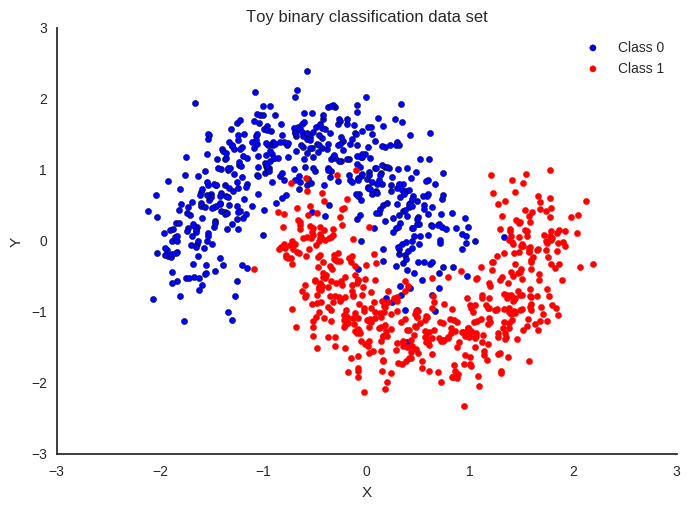
\includegraphics[width=12cm]{figures/1174084/2/1.png}
    \centering
    \caption{gambaran binary classification}
\end{figure}
	\hfill\\
Klasifikasi biner atau binomial adalah tugas mengklasifikasikan elemen-elemen dari himpunan yang diberikan ke dalam dua kelompok (memprediksi kelompok mana yang masing-masing dimiliki) berdasarkan aturan klasifikasi. 

\item Jelaskan Apa itu supervised learning , unsupervised learning dan clusterring dengan ilustrasi gambar
\begin{enumerate}
\item supervised learning
	\hfill\\
	Dalam bahasa indonesia Supervised Learning adalah pembelajaran yang ada supervisornya. Maksud ada supervisornya adalah label di tiap data nya. Label adalah tag dari data yang ditambahkan dalam machine learning model. Contohnya gambar kucing di tag “kucing” di tiap masing masing image kucing dan gambar anjing di tag “anjing” di tiap masing gambar anjing. Machine learning kategori berupa clasification (“anjing”, “kucing”, “beruang”, dsb) dan regression ( berat badan, tinggi badan dsb). Supervised learning digunakan untuk memprediksi pola yang sudah ada contoh data yang lengkap, jadi pola yang terbentuk adalah hasil pembelajaran data lengkap tersebut. Jika kita memasukan data baru, setelah melakukan ETL (Extract Transform Load) maka kita mendapat info feature dari sample baru tersebut. Kemudian feature tersebut di compare dengan pattern clasification dari model yang didapat dari label data. Setiap label di compare hingga selesai, dan yang memiliki percentage lebih banyak akan diambil sebagai prediksi akhir.

\begin{figure}[H]
    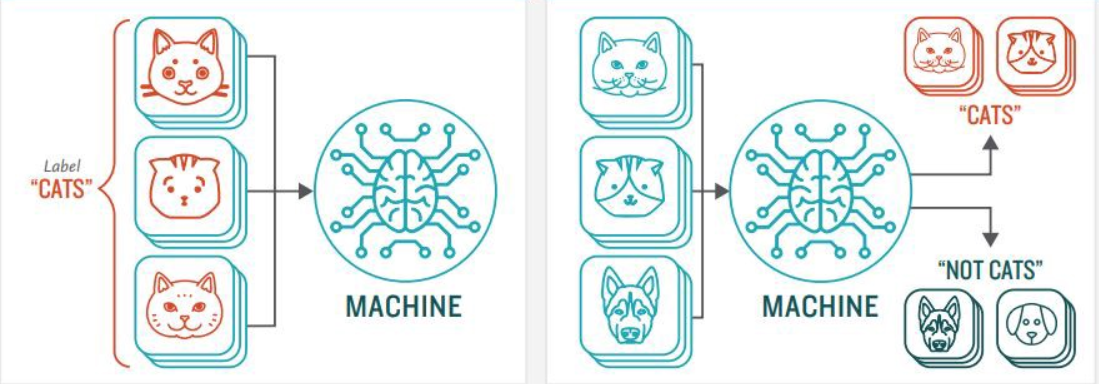
\includegraphics[width=12cm]{figures/1174084/2/2.png}
    \centering
    \caption{gambaran cara kerja supervised}
\end{figure}

\item unspervised learning
	\hfill\\
	Unsupervised learning tidak menggunakan label seperti supervised learning dalam memprediksi target feautures / variable. Melainkan menggunakan ke samaan dari attribut attribut yang dimiliki. Apabila attribut dan sifat-sifat dari data data feature yang diekstrak memiliki kemirip-miripan, maka akan dikelompok-kelompokan (clustering). Sehingga hal ini akan menimbulkan kelompok-kelompok (cluster). Jumlah cluster bisa unlimited. Dari kelompok itu model melabelkan, dan jika data baru mau di prediksi, maka akan dicocokkan dengan kelompok yang mirip dengan featurenya.
\begin{figure}[H]
    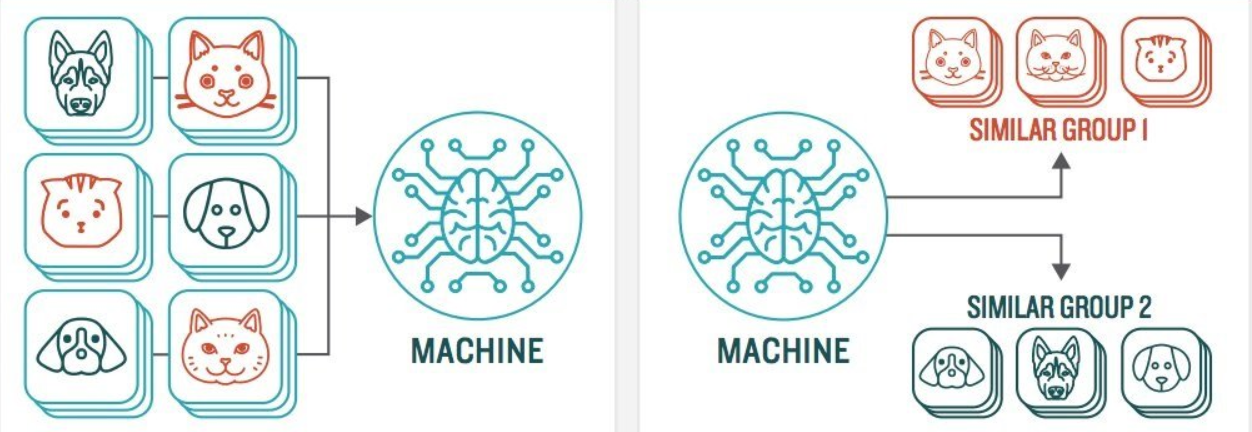
\includegraphics[width=12cm]{figures/1174084/2/3.png}
    \centering
    \caption{gambaran cara kerja unsupervised}
\end{figure}

\item Clustering 
	\hfill\\
	Clustering adalah sebuah metode untuk membedakan data - data menjadi kumpulan dari group yang isinya merupakan data yang serupa setiap grupnya. Basisnya dapat berupa kesamaan atau perbedaan dari setiap grup tersebut.
\begin{figure}[H]
    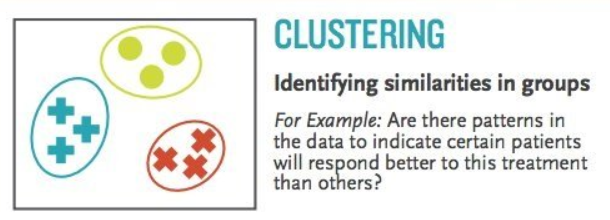
\includegraphics[width=12cm]{figures/1174084/2/4.png}
    \centering
    \caption{gambaran clustering}
\end{figure}
\end{enumerate}
\item Jelaskan apa itu evaluasi dan akurasi dan disertai ilustrasi contoh dengan gambar
	\hfill\\
	Evaluasi adalah tentang bagaimana kita dapat mengevaluasi seberapa baik model bekerja dengan mengukur akurasinya. Dan akurasi akan didefinisikan sebagai persentase kasus yang diklasifikasikan dengan benar. Kita dapat menganalisis kesalahan yang dibuat oleh model,atau tingkat kebingungannya,menggunakan matriks kebingungan(\textit{confusion matrix}). Matriks kebingungan mengacu pada kebingungan dalam model,tetapi matriks kebingungan ini bisa menjadi sedikit sulit untuk dipahami ketika mereka menjadi sangat besar.
\begin{figure}[H]
    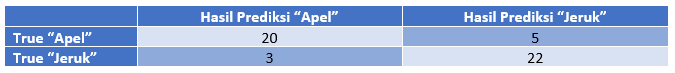
\includegraphics[width=12cm]{figures/1174084/2/5.png}
    \centering
    \caption{contoh confusion matrix}
\end{figure}

\item Jelaskan bagaimana cara membuat Confusion Matrix, Buat confusion matrix
\hfill\\
	Confusion matrix juga sering disebut error matrix. Pada umumnya confusion matrix memberikan informasi perbandingan hasil klasifikasi yang dilakukan oleh sistem (model) dengan hasil klasifikasi sebenarnya. Confusion matrix berbentuk tabel matriks yang menggambarkan kinerja model klasifikasi pada serangkaian data uji yang nilai sebenarnya diketahui. Untuk menggunakan Confusion Matrix, ada 4 istilah sebagai hasil proses dari klasifikasi. Diantaranya adalah :
\begin{itemize}
    \item True Positive : Data positif yang terdeteksi memiliki hasil benar
    \item False Positive : Data Positif yang terdeteksi memiliki hasil salah
    \item True Negative : Data negatif yang terdeteksi memiliki hasil benar
    \item False Negative : Data negatif yang terdeteksi memiliki hasil salah
\end{itemize}
\begin{figure}[H]
    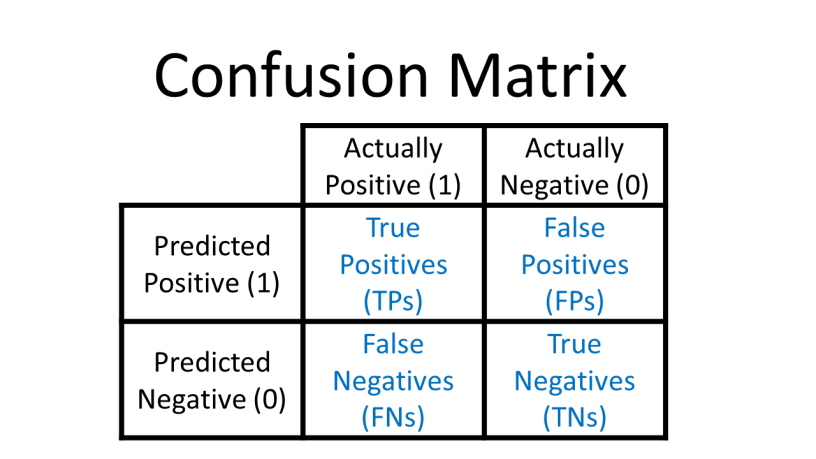
\includegraphics[width=12cm]{figures/1174084/2/6.png}
    \centering
    \caption{contoh confusion matrix}
\end{figure}	

\item Jelaskan bagaimana K-fold cross validation bekerja dengan gambar ilustrasi contoh
	\hfill\\
Cara kerja k-fold validation:
\begin{itemize}
	\item Total instance dibagi menjadi N bagian.
	\item Fold yang pertama adalah bagian pertama menjadi data uji (testing data) dan sisanya menjadi training data.
	\item Lalu hitung akurasi berdasarkan porsi data tersebut dengan menggunakan persamaan.
	\item Fold yang kedua adalah bagian kedua, yang menjadi data uji(testing data)dan sisanya training  data.
	\item Kemudian hitung akurasi berdasarkan porsi data tersebut.
	\item Dan seterusnya hingga habis mencapai fold ke-K.
	\item Terakhir hitung rata-rata akurasi K buah.
\end{itemize}
\begin{figure}[H]
    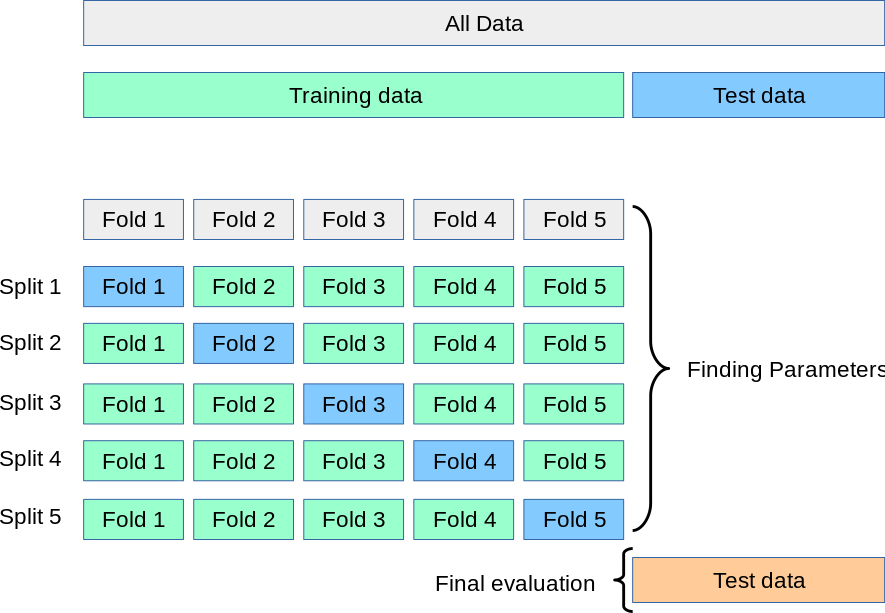
\includegraphics[width=8cm]{figures/1174084/2/7.png}
    \centering
    \caption{contoh K-Fold Validation}
\end{figure}

\item Jelaskan Apa itu decision tree dengan gambar ilustrasi contoh buatan sendiri.
	\hfill\\
	Decision tree merupakan model prediksi menggunakan struktur pohon atau struktur berhirarki. Hasil dari setiap struktur biasanya menggunakan jawaban (True dan False) atau cabang lain yang akan menjadi pohon selanjutnya. Setiap keputusan diantaranya akan membandingkan kondisi yang diberikan kepada struktur untuk dibandingkan kondisi apa saja yang sudah didapat pada sistem tersebut.
\begin{figure}[H]
    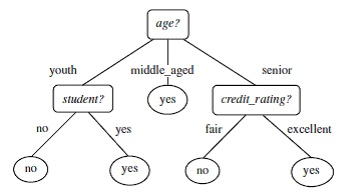
\includegraphics[width=8cm]{figures/1174084/2/8.png}
    \centering
    \caption{Decision Tree}
\end{figure}


\item jelaskan apa itu information gain dan entropi dengan gambar ilustrasi

\begin{enumerate}
	\item information Gain
	\hfill\\
	Information Gain adalah teknik seleksi fitur dengan cara memakai metode scoring untuk nominal ataupun pembobotan atribut kontinu yang didiskretkan menggunakan maksimal entropy. Suatu entropy digunakan untuk mendefinisikan nilai Information Gain. Entropy menggambarkan banyaknya informasi yang dibutuhkan untuk mengkodekan suatu kelas 
\begin{figure}[H]
    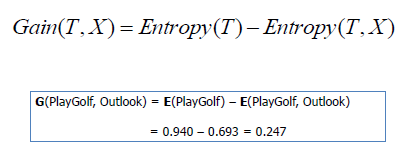
\includegraphics[width=12cm]{figures/1174084/2/9.png}
    \centering
    \caption{information gain}
\end{figure}

	\item Entropi
	\hfill\\
	Entropi merupakan pengukuran sebuah data dan validnya data tersebut untuk dapat digunakan sebagai informasi yang akan dimasukkan ke Information Gain. Entropi menilai sebuah obyek berdasarkan kebutuhan di dunia nyata dan pengaruh pada sistem yang akan digunakan.
\begin{figure}[H]
    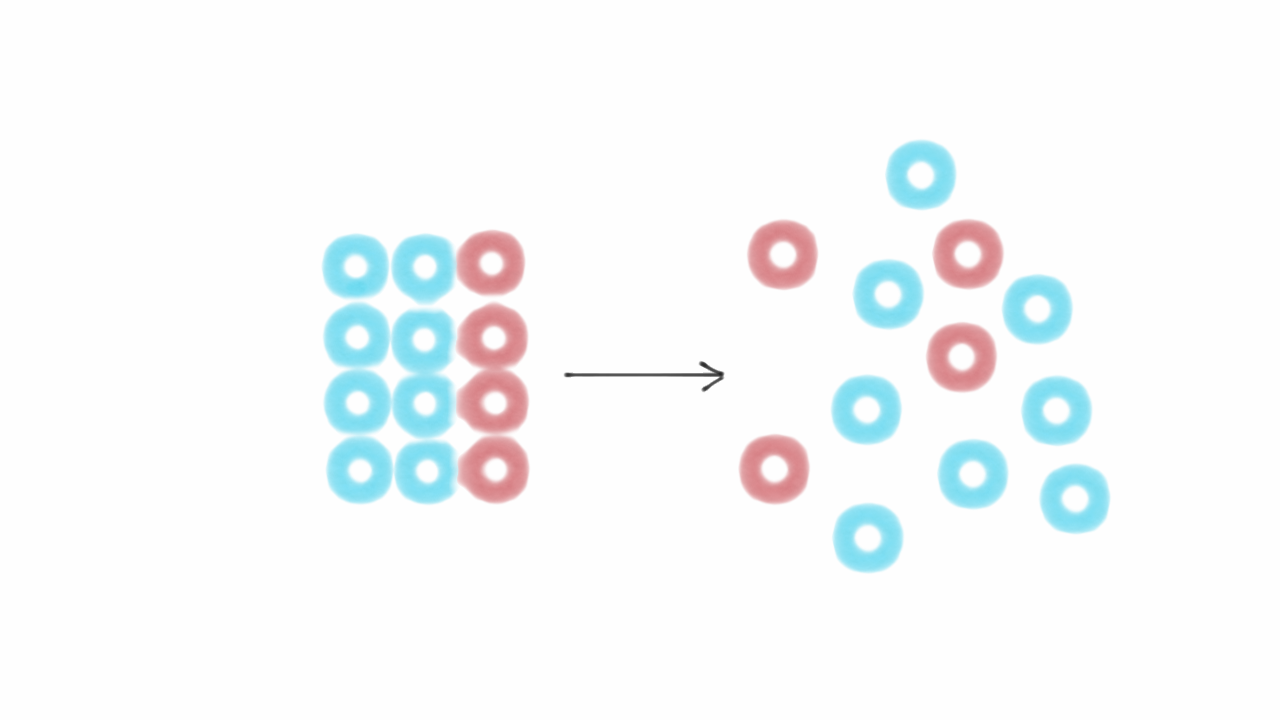
\includegraphics[width=8cm]{figures/1174084/2/10.png}
    \centering
    \caption{penggambaran entropi}
\end{figure}
\end{enumerate}
\end{enumerate}



\subsection{Praktek}
	Tugas anda adalah, dataset ganti menggunakan student-mat.csv dan mengganti semua nama variabel dari kode di bawah ini dengan nama-nama makanan (NPM mod 3=0), kota (NPM mod 3=1), buah (NPM mod 3=2),
\lstinputlisting[firstline=9, lastline=12]{src/1174084/2/1174084.py} 
\begin{enumerate}
\item No. 1
	\hfill\\
	\lstinputlisting[firstline=13, lastline=18]{src/1174084/2/1174084.py}
\begin{figure}[H]
    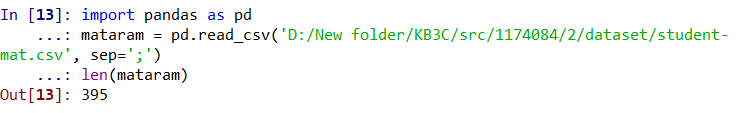
\includegraphics[width=8cm]{figures/1174084/2/praktek/1.png}
    \centering
    \caption{Loading Dataset}
\end{figure}

\item No. 2
	\hfill\\
	\lstinputlisting[firstline=19, lastline=24]{src/1174084/2/1174084.py}
\begin{figure}[H]
    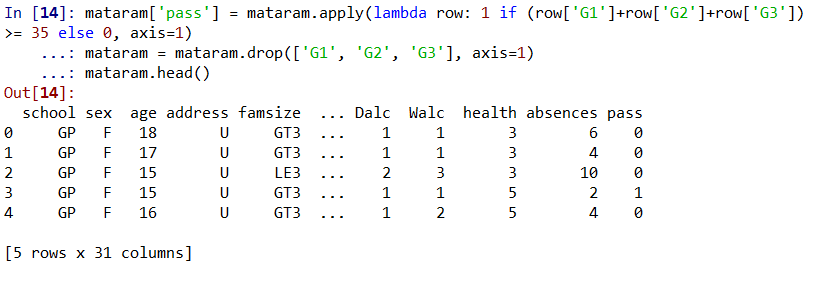
\includegraphics[width=8cm]{figures/1174084/2/praktek/2.png}
    \centering
    \caption{Generate Binary Label}
\end{figure}

\item No. 3
	\hfill\\
	\lstinputlisting[firstline=25, lastline=31]{src/1174084/2/1174084.py}
\begin{figure}[H]
    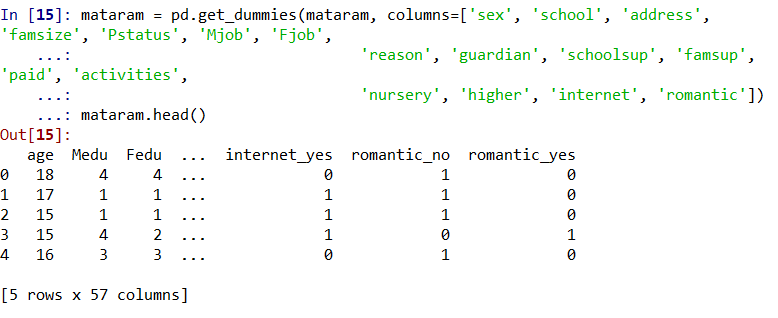
\includegraphics[width=8cm]{figures/1174084/2/praktek/3.png}
    \centering
    \caption{One-hot Encoding}
\end{figure}

\item No. 4
	\hfill\\
	\lstinputlisting[firstline=32, lastline=51]{src/1174084/2/1174084.py}
\begin{figure}[H]
    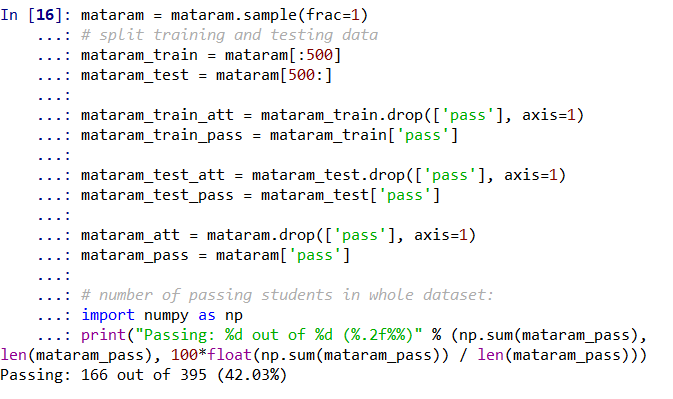
\includegraphics[width=8cm]{figures/1174084/2/praktek/4.png}
    \centering
    \caption{Shuffle Rows}
\end{figure}

\item No. 5
	\hfill\\
	\lstinputlisting[firstline=53, lastline=58]{src/1174084/2/1174084.py}
\begin{figure}[H]
    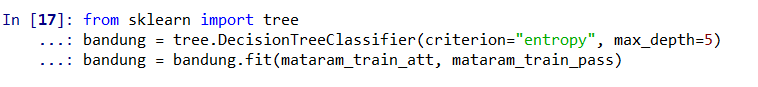
\includegraphics[width=8cm]{figures/1174084/2/praktek/5.png}
    \centering
    \caption{Fit Decision tree}
\end{figure}

\item No. 6
	\hfill\\
	\lstinputlisting[firstline=59, lastline=69]{src/1174084/2/1174084.py}
\begin{figure}[H]
    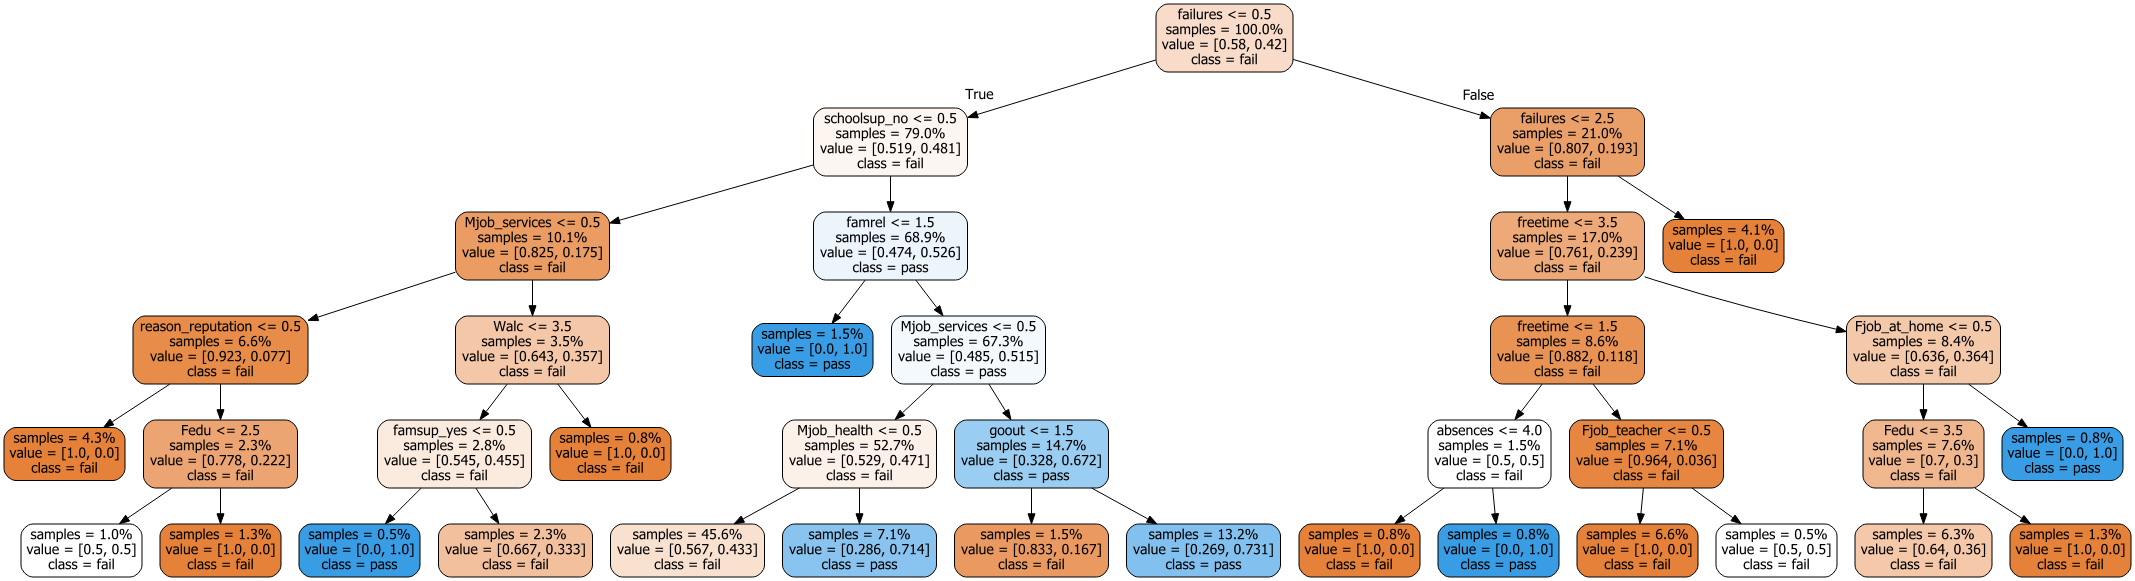
\includegraphics[width=12cm]{figures/1174084/2/praktek/6.png}
    \centering
    \caption{Visualize tree}
\end{figure}

\item No. 7
	\hfill\\
	\lstinputlisting[firstline=70, lastline=75]{src/1174084/2/1174084.py}
\begin{figure}[H]
    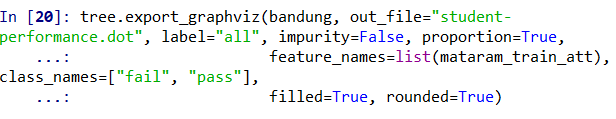
\includegraphics[width=8cm]{figures/1174084/2/praktek/7.png}
    \centering
    \caption{menyimpan(save) tree}
\end{figure}

\item No. 8
	\lstinputlisting[firstline=76, lastline=79]{src/1174084/2/1174084.py}

\item No. 9
	\hfill\\
	\lstinputlisting[firstline=80, lastline=85]{src/1174084/2/1174084.py}
\begin{figure}[H]
    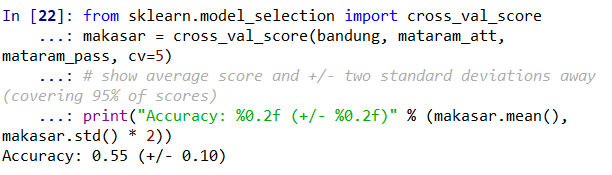
\includegraphics[width=8cm]{figures/1174084/2/praktek/9.png}
    \centering
    \caption{Cross Val Score}
\end{figure}

\item No. 10
	\hfill\\
	\lstinputlisting[firstline=87, lastline=92]{src/1174084/2/1174084.py}
\begin{figure}[H]
    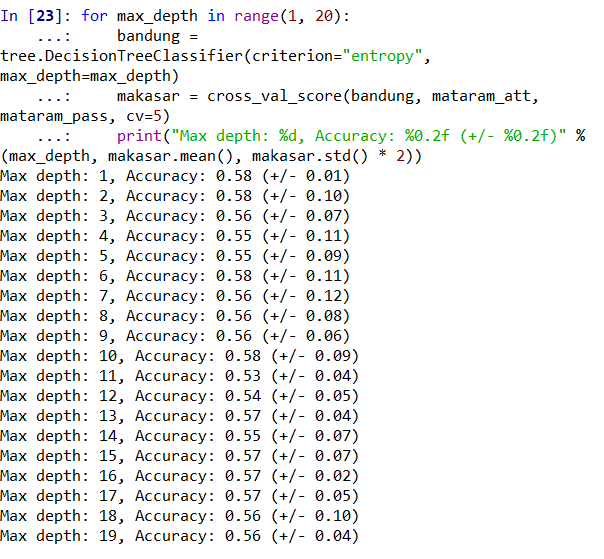
\includegraphics[width=8cm]{figures/1174084/2/praktek/10.png}
    \centering
    \caption{Max Depth}
\end{figure}

\item No. 11
	\hfill\\
	\lstinputlisting[firstline=93, lastline=104]{src/1174084/2/1174084.py}
\begin{figure}[H]
    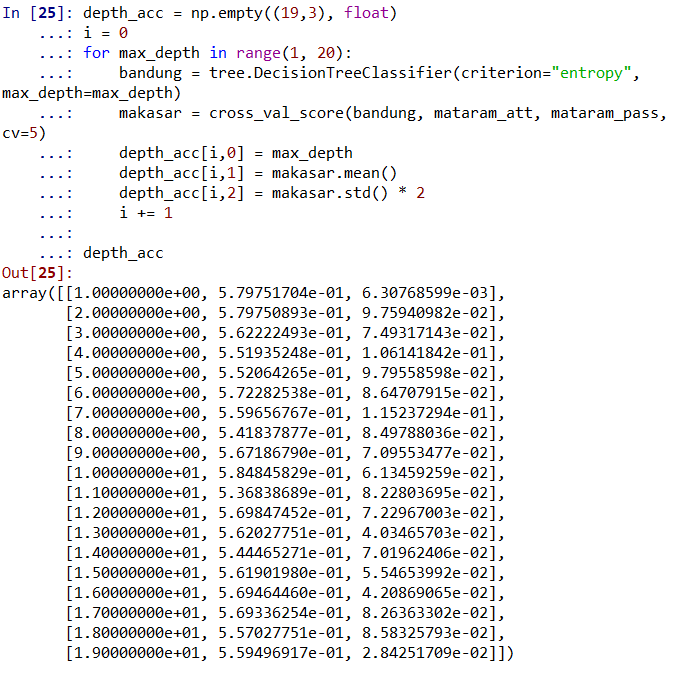
\includegraphics[width=8cm]{figures/1174084/2/praktek/11.png}
    \centering
    \caption{Depth in Range}
\end{figure}

\item No. 12
	\hfill\\
	\lstinputlisting[firstline=106, lastline=111]{src/1174084/2/1174084.py}
\begin{figure}[H]
    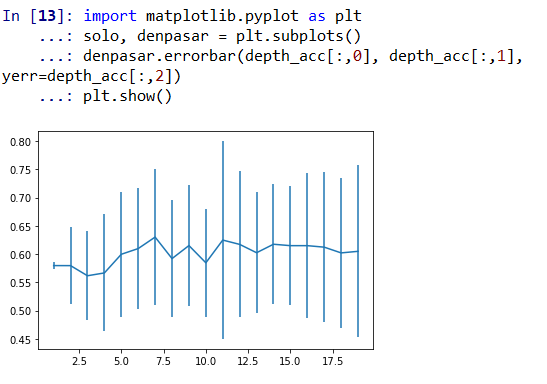
\includegraphics[width=8cm]{figures/1174084/2/praktek/12.png}
    \centering
    \caption{Matplotlib}
\end{figure}
\end{enumerate}

\subsection{Penanganan Error}
\begin{enumerate}
\item Error
\begin{figure}[H]
    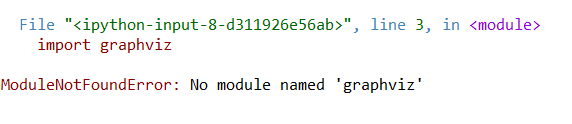
\includegraphics[width=8cm]{figures/1174084/2/error/1.png}
    \centering
    \caption{No module named graphviz}
\end{figure}
\item Solusi: 
	\begin{figure}[H]
    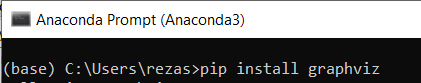
\includegraphics[width=8cm]{figures/1174084/2/error/2.png}
    \centering
    \caption{Solusi dengan anaconda promt}
	\end{figure}

\end{enumerate}

\subsection{Bukti Tidak Plagiat}
\begin{figure}[H]
	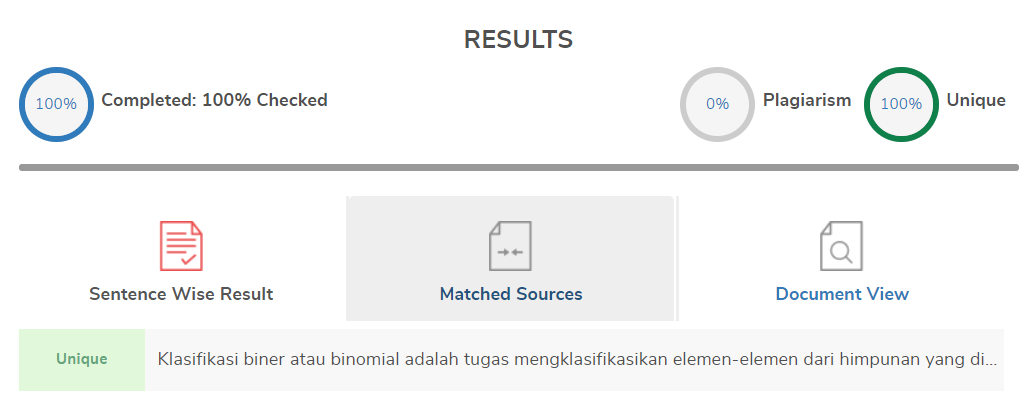
\includegraphics[width=4cm]{figures/1174084/2/plagiarism.png}
	\centering
	\caption{plagirism}
\end{figure}


\subsection{Link Video Youtube}
https://youtu.be/7gIPgpQA1LA
